% This LaTeX was auto-generated from MATLAB code.
% To make changes, update the MATLAB code and export to LaTeX again.

\documentclass{article}

\usepackage[utf8]{inputenc}
\usepackage[T1]{fontenc}
\usepackage{lmodern}
\usepackage{graphicx}
\usepackage{color}
\usepackage{hyperref}
\usepackage{amsmath}
\usepackage{amsfonts}
\usepackage{epstopdf}
\usepackage[table]{xcolor}
\usepackage{matlab}

\sloppy
\epstopdfsetup{outdir=./}
\graphicspath{ {./phenomenology_images/} }

\begin{document}

\label{H_F310D61F}
\matlabtitle{Phenomenological calculations}


\vspace{1em}
\matlabheading{Flux density}

\begin{par}
\begin{flushleft}
Flux densities are calculated using \texttt{fluxdensitySquare(lpd, b, a, x, y)}\textit{ }and \texttt{fluxdensitySquare(lpd, b, a, x, y)}.
\end{flushleft}
\end{par}

\begin{par}
\begin{flushleft}
\texttt{lpd - London's penetration depth}
\end{flushleft}
\end{par}

\begin{par}
\begin{flushleft}
\texttt{b - Magnetic field strength}
\end{flushleft}
\end{par}

\begin{par}
\begin{flushleft}
\texttt{a - Lattice constant}
\end{flushleft}
\end{par}

\begin{par}
\begin{flushleft}
\texttt{x,y - Coordinates, can be scalar or mesh of coordinates }
\end{flushleft}
\end{par}


\vspace{1em}
\begin{par}
\begin{flushleft}
\texttt{dataHexCode.m }and\texttt{ dataSquareCode.m }is used to generate flux density data \texttt{datahex.mat} and \texttt{datasquare.mat} in hexagonal and square lattice respectively.
\end{flushleft}
\end{par}

\begin{par}
\begin{flushleft}
In the following codes, generated data were imported and plotted.
\end{flushleft}
\end{par}

\begin{par}
\begin{flushleft}
Flux density of the square lattice:
\end{flushleft}
\end{par}

\begin{matlabcode}
run("fluxPlotSquare.m")
\end{matlabcode}
\begin{center}
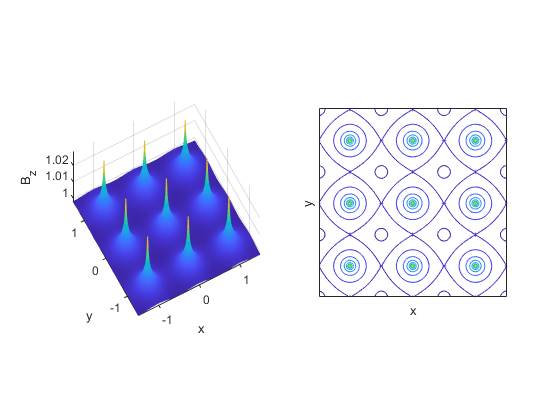
\includegraphics[width=\maxwidth{56.196688409433015em}]{figure_0.png}
\end{center}

\begin{par}
\begin{flushleft}
Flux density of the hexagonal lattice:
\end{flushleft}
\end{par}

\begin{matlabcode}
run('fluxPlotHex.m')
\end{matlabcode}
\begin{center}
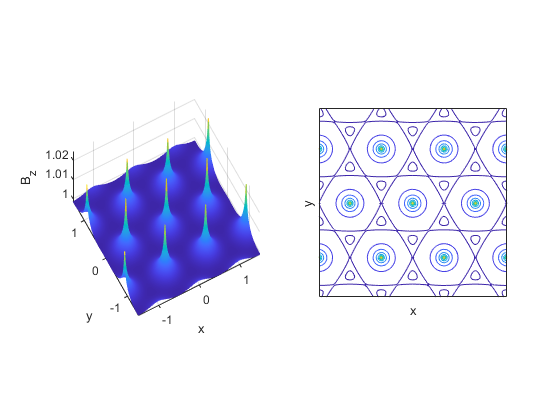
\includegraphics[width=\maxwidth{56.196688409433015em}]{figure_1.png}
\end{center}

\begin{par}
\begin{flushleft}
Flux histogram of hexagonal lattice:
\end{flushleft}
\end{par}

\begin{matlabcode}
run('fluxPlotHistogram.m')
\end{matlabcode}
\begin{matlaboutput}
Warning: Class 'Annotate' uses an undocumented syntax to restrict property values. Use property validation syntax instead. This warning will become an error in a future release.
\end{matlaboutput}
\begin{center}
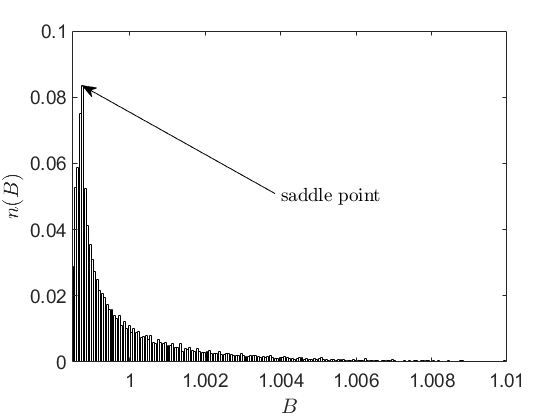
\includegraphics[width=\maxwidth{56.196688409433015em}]{figure_2.png}
\end{center}


\vspace{1em}
\matlabheading{Free energy}

\begin{par}
\begin{flushleft}
Free energy are calculated using \texttt{freeEnergyHex(a, b, lpd, N) }and \texttt{freeEnergySquare(a, b, lpd, N)}.
\end{flushleft}
\end{par}

\begin{par}
\begin{flushleft}
\texttt{lpd - London's penetration depth}
\end{flushleft}
\end{par}

\begin{par}
\begin{flushleft}
\texttt{b - Magnetic field strength}
\end{flushleft}
\end{par}

\begin{par}
\begin{flushleft}
\texttt{a - Lattice constant}
\end{flushleft}
\end{par}

\begin{par}
\begin{flushleft}
\texttt{N - Lattice length (for one side, i.e. size is N*N)}
\end{flushleft}
\end{par}


\vspace{1em}
\begin{par}
\begin{flushleft}
\texttt{freeenergy.m }is used to generate struct for energy of both hexagonal and square lattice in different lattice length \texttt{N}.
\end{flushleft}
\end{par}

\begin{par}
\begin{flushleft}
Plot source code:
\end{flushleft}
\end{par}

\begin{matlabcode}
run("freeEnergyPlot.m")
\end{matlabcode}
\begin{center}
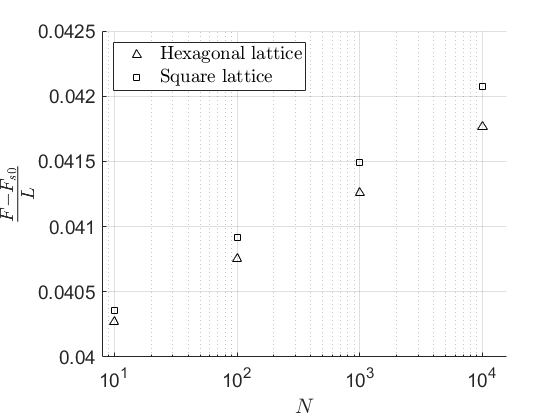
\includegraphics[width=\maxwidth{56.196688409433015em}]{figure_3.png}
\end{center}

\matlabheading{Supercurrent}

\begin{par}
\begin{flushleft}
Supercurrent are calculated using\texttt{ currentSquare(lpd, b, a, x, y)}.
\end{flushleft}
\end{par}

\begin{par}
\begin{flushleft}
\texttt{lpd - London's penetration depth}
\end{flushleft}
\end{par}

\begin{par}
\begin{flushleft}
\texttt{b - Magnetic field strength}
\end{flushleft}
\end{par}

\begin{par}
\begin{flushleft}
\texttt{a - Lattice constant}
\end{flushleft}
\end{par}

\begin{par}
\begin{flushleft}
\texttt{x,y - Coordinates, can be scalar or mesh of coordinates }
\end{flushleft}
\end{par}


\vspace{1em}
\begin{par}
\begin{flushleft}
\texttt{dataCurrentSquareCode.m }is used to generate flux density data \texttt{datacurrentsquare.mat} in square lattice.
\end{flushleft}
\end{par}

\begin{par}
\begin{flushleft}
Plot source code:
\end{flushleft}
\end{par}

\begin{matlabcode}
run('currentSquarePlot.m')
\end{matlabcode}
\begin{matlaboutput}
Warning: Using only the real component of complex data.
\end{matlaboutput}
\begin{center}
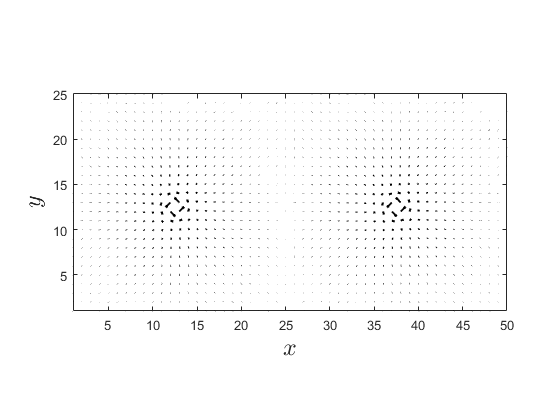
\includegraphics[width=\maxwidth{56.196688409433015em}]{figure_4.png}
\end{center}

\end{document}
